\item A small body \( A \) starts sliding off the top of a smooth sphere of radius \( R \). Find the angle \( \theta \) (Fig. 1.25) corresponding to the point at which the body breaks off the sphere, as well as the break-off velocity of the body.
    \begin{center}
        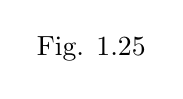
\begin{tikzpicture}
            \node at (0, 0) {Fig. 1.25};
        \end{tikzpicture}
    \end{center}\begin{solution}
    \begin{center}
        \begin{tikzpicture}
            \pic at (0, 0) {frame=3cm};
        \end{tikzpicture}
    \end{center}
 
    \begin{align*}
        &\intertext{Let us depict the forces acting on the body $A$ (which are the force of gravity $mg$ and the normal reaction $N$) and write equation $\vec{F} = m \vec{w}$ via projection on the unit vectors $\vec{t}$ and $\vec{n}$ (see figure).}
        &\text{From } F_t =mv_t\\
        &mg\sin{\theta} = m \dfrac{dv}{dt}\\
        &= m v \dfrac{dv}{ds} = m \dfrac{vdv}{R d\theta}\\
        &\text{or} \quad g R \sin{\theta} d \theta = v dv\\
        &\intertext{Integrating both sides for obtaining $v(\theta)$, we get}
        &\int_0^{\theta} g R \sin \theta' \, d \theta' = \int_0^v v \, dv\\
        &\text{or} \quad v^2 = 2 g R \left(1 - \cos{\theta}\right) \tag{1}\\
        &\text{From } F_n =m v_n\\
        &mg \cos{\theta} - N = m \dfrac{v^2}{R} \tag{2}\\
        &\intertext{At the moment the body loses contact with the surface, $N=0$, and therefore Eq. (2) becomes}
        &v^2 = g R \cos \theta \tag{3}\\
        &\text{where $v$ and $\theta$ correspond to the moment when the body loses contact with the surface. Solving Eqs. (1) and (3), we obtain}\\
        &\cos \theta = \dfrac{2}{3} \quad \text{or} \quad \theta = \cos^{-1} (2/3) \approx 48^\circ \quad \text{and} \quad v = \sqrt{\dfrac{2 g R}{3}}
    \end{align*}
\end{solution}